\documentclass[9pt, twocolumn, compsoc]{IEEEtran}
\input{preamble_ieee.tex}
\usepackage{mathtools}
\usepackage{flushend}
%####################################
\title{NERO: Non-parametric Entropy-rate Oracle to Recognize AI-Generated Content % Computing Entropy Rate Of Symbol Sources \\ \& A Distribution-free Limit Theorem
} 
\author{
\begin{tabular}{cc}
Kevin Wu, Hod Lipson and Ishanu Chattopadhyay$^\star$\\ $^\star$Corresponding Author: ishanu@uchicago.edu
\end{tabular}
}
\begin{document}  
\maketitle 
\begin{abstract}
Entropy rate of sequential data-streams naturally quantifies the  complexity of the generative process. Thus entropy rate fluctuations   could be used as a  tool to recognize  dynamical perturbations in  signal sources, and could  potentially be carried out without explicit   background noise characterization. However, state of the art algorithms to estimate the entropy rate have markedly slow convergence; making such entropic approaches non-viable in practice. We present here a fundamentally new approach to estimate entropy rates, which is demonstrated to converge significantly faster in terms of input data lengths, and is shown to be effective in diverse applications ranging from the estimation of the  entropy rate of English texts to the estimation of  complexity of chaotic dynamical systems. Additionally, the convergence rate of  entropy estimates  do not follow from any standard limit theorem, and reported algorithms  fail to provide  any  confidence bounds on the computed values.  Exploiting a connection to the theory of probabilistic automata, we establish a  convergence rate of $O(\log \vert s \vert/\sqrt[3]{\vert s \vert})$ as a function of the input length $\vert s \vert$,  which then   yields explicit  uncertainty estimates, as well as  required  data lengths to satisfy pre-specified confidence bounds.  
\end{abstract}
\begin{IEEEkeywords} 
 Entropy rate, Stochastic processes, Probabilistic  automata,  Symbolic dynamics
\end{IEEEkeywords}
%\abbreviations{SSA, Gillespie's Stochastic Simulation Algorithm; RP, Reaction Polytope; LV, Lotka-Volterra prey-predator stochastic reaction system}
% % ###########################################################
% % END PREAMBLE ##############################################
% #############################################################
\allowdisplaybreaks{ 
%##############################################################
% 
% The paper is summarized and concluded in Section~\ref{sec6}.
% % ##################################################
% % #######################################################
% % #######################################################
% \section{Entropy Rate of Stochastic Processes}
% \subsection{Contribution}
  \section*{Introduction}


  \section*{Results}

  \section*{Discussion}

  \section*{Methods}
  
\subsection*{Efficiently Computing Entropy Rate Of Symbol Sources}
The entropy rate of a stationary and ergodic process converges in probability to the  per-letter Kolmogorov complexity of a single sufficiently long sample path~\cite{horibe03}. While  Kolmogorov complexity is incomputable, entropy rates  can, in principle, be estimated. Ability to quantify  the complexity of a signal source, even in the average sense,  can provide valuable insights into the driving dynamics; and can potentially be used as a  tool to detect dynamical anomalies without explicit knowledge of  background noise processes.

However,  source entropy rate estimation  from an observed sample path is computationally non-trivial. Even with the assumptions of ergodicity and stationarity, one cannot fruitfully apply the defining relation in Eq.\eqref{eqentropy} due to the exponential increase in the number of different words with the word-length. This is particularly important  if there are long-range dependencies in the symbol stream.  Such dependencies introduce additional long-range structure; decreasing the source entropy  in the process. In such cases  unacceptably long words or \textit{blocks} must be considered, and pre-mature truncation of the computation would lead to large errors. 

 The best known algorithms  that carry out a  more efficient  computation are based on  Lempel-Ziv (LZ) source coding~\cite{LZ77,LZ78,LZ77opt}. The LZ coding algorithms are asymptotically optimal, $i.e.$ their compression rate approaches the source entropy rate for any ergodic stationary stochastic process. The key idea here is adaptive dictionary compression: parse the input string into distinct phrases, and represent them with codewords, making sure that  short codewords are assigned to common phrases. Done optimally, one ends up with a compressed string, such that the ratio of the input and output lengths approach the source entropy rate. Different variations on this idea have been reported~\cite{langdon83,grassberger89}. Techniques distinct from  LZ parsing  are also known, $e.g.$,  Rissanen~\cite{rissanen83} reported a universal compression scheme, which instead of gathering parsed segments of the input along with their occurrence counts, collects  the ``contexts'' in which each symbol of  the  input string  occurs, together with   conditional  occurrence counts.

Importantly, a majority of the reported techniques do more than just compute the entropy rate; they are indeed full-scale data compression utilities, that produce a decodable representation of the input. Can we do better if we are only interested in the former? This paper provides an affirmative answer to this possibility.

Secondly,  existing techniques lack convergence rate estimates; computation of error bars for reported approaches do not follow from any standard limit theorem. There is indeed no analytical way to check for the internal consistency of
the estimation or its accuracy. We may observe gradual convergence to a limiting value, and this is indeed guaranteed by theory;  but  are unable to  provide uncertainty bounds on the computed  estimate with finite inputs. Typically observed slow convergence in all non-trivial scenarios, for all reported algorithms,  makes this a key issue. An empirical relationship, without proof or theoretical backing, has been suggested~\cite{shgs96}, which conjectures the $\vert s \vert$-dependence ($\vert s \vert$ being the length of the input $s$) of the estimated entropy rate $\widetilde{H}$ to follow
%\cgather{ 
$\widetilde{H} \simeq H_{actual} + c \frac{\log \vert s \vert}{\vert s \vert^\gamma}, \textrm{where } c,\gamma \textrm{ are fit parameters}$. 
%}
In this paper, we show that, at least with our algorithm, the convergence rate is given by $O(\log \vert s \vert / \sqrt[3]{\vert s \vert})$. This is a distribution-free result, in the sense that the asymptotic  bound does not depend on the source characteristics. In consequence, we can derive explicit uncertainty estimates at specified  confidence bounds on the estimated entropy rate for finite-length input data.

% #######################################
% #######################################
\begin{figure}[t]
\tikzexternalenable
\centering
 %\newcommand{\VSP}{\rule{0pt}{1.75ex}}
 \begin{tikzpicture}[,font=\bf\fontsize{8}{8}\selectfont,->,>=latex',shorten >=1pt,auto,node distance=1.2cm,  scale=1 ,]
  \node [circle, draw=black, dashed, thick ] (A) at (0.15,1.5) [align=center]{\bf Hidden\\\bf Process};
\draw [fill=lightgray,draw=none,opacity=.9, xslant=0.0,yslant=.4, path fading=east] (0,0) -- (1.5,0) -- (1.5,2.5) -- (0,2.5) -- cycle;  
\draw [xshift=-.8in,yshift=.275in,fill=lightgray,draw=none,opacity=.9, xslant=0.0,yslant=-.35, path fading=west] (0,0) -- (2,0) -- (2,2.5) -- (0,2.5) -- cycle;  
\draw [xshift=-.635in,yshift=1.225in,fill=lightgray,draw=none,opacity=1, xslant=2.45,yslant=-.19, path fading=west] (0,0) -- (3,0) -- (3,.5) -- (0,.5) -- cycle; 

%\draw [fill=gray,draw=none,opacity=1, path fading=south ,
%xslant=0.0,yslant=.4] (0,-1) -- (2,-1) -- (2,-.2) -- (0,-.2) -- cycle;

    \node [anchor=west] (B) at (A.east) [align=center]{\bf 01010010101011100101010101010$\boldsymbol{\cdots}$};
   \node [anchor=north, text=Red4] (C) at ([yshift=-.1in]B.south) [align=left]{\textbullet~Entropy rate?};
   \node [anchor=north west, text=Red4] (C1) at ([yshift=0.07in]C.south west) [align=left]{\textbullet~Convergence Rate of estimate?};  
 \node [anchor=south, text=gray] (C) at (B.north) [align=center]{States are\\ hidden};
   \node [anchor=north east,text=gray,font=\bf\fontsize{7}{8}\selectfont] (D) at ([yshift=.45in,xshift=-.1in]A.south west) [align=center]{ Stationary\\ergodic\\stochastic\\process};
\end{tikzpicture} 

\vspace{-5pt}

\captionN{\textbf{Problem description.} Given a quantized data stream, how do we compute the entropy rate of the hidden  process? Even with the  assumption of  stationarity and ergodicity for  the generator, reported algorithms converge very slowly. Additionally,  these convergence rates are unknown for such approaches; implying that we cannot put uncertainty bounds on the computed values in practice. We show that a significantly faster computation of the entropy rate is possible; and derive a universal lower bound on how slowly this convergence might occur.
}\label{figstrm}
\vspace{-12pt}

\end{figure}
% #######################################
% #######################################
\subsubsection*{Key Insight}
Our approach is based on  modeling discrete and finite-valued stationary and ergodic sources as probabilistic automata. Our automata is distinct from that of Paz~\cite{P71}, and each model in our case is  in fact an  encoding of a measure defined on the space of  strictly infinite strings over a finite alphabet. While the formalisms are  completely different, some aspects of this approach has subtle parallels to that of Rissanen's ``context algorithm''~\cite{rissanen83}; his search for contexts which yield similar probabilities of generating future symbols is analogous to our search for a synchronizing string in the input stream - a finite sequence of symbols that, once executed on a probabilistic automaton, leads to a fixed state irrespective of the initial conditions. Of course we do not know anything about the hidden model a priori; but nevertheless we establish that such a string, at least in a well-defined approximate sense, always exists and is identifiable efficiently. Finally, we show that, given such an approximate synchronizing string, we can use results from non-parametric statistics to bound the probability of error as a function of the input length.
\subsubsection*{Entropy  \& Entropy Rate}
Entropy $H(X)$ of a discrete random variable $X$, taking values in the alphabet $\Sigma$,  is defined as:
\cgather{
H(X) = - \sum_{x \in \Sigma} p(x)\log p(x)
}where $p(x)$ is the probability of occurrence of $x \in \Sigma$. 
The base of the logarithm is generally taken to be $2$, and then the entropy is being expressed in \textit{bits}. While the definition of entropy of a random variable may be obtained axiomatically, a perhaps more compelling  approach is to show that it arises 
as the average length of the shortest description of a random variable~\cite{cover}.

The joint entropy of a set of random variables $X_1,\cdots,X_n$, with $X_i$  taking values in the alphabet $\Sigma_i$, is defined in the usual manner: 
\cgather{
H(X_1,\cdots,X_n) = - \sum_{x_i \in \Sigma_i} p(x_1,\cdots, x_n) \log_2 p(x_1,\cdots, x_n) 
}
% The conditional entropy of a random variable is  the expected entropy of the conditional distributions:
% \cgather{
% H(Y\vert X)  =  \sum_{x \in \Sigma} p(x) H(Y\vert X=x)
% }
The chain rule for entropy calculations~\cite{cover} follows from the definitions, and is of particular importance:
\cgather{\label{eqchrule}
H(X_1,\cdots,X_n)= \sum_{i=1}^n H(X_i \vert X_{i-1},\cdots,X_1)
}
The notion of entropy formalizes the Asymptotic Equipartion Property (AEP): If discrete random variables  $X_1,\cdots, X_n$ are i.i.d. and have probability mass function $p(x)$, then we have:
\cgather{
-\frac{1}{n} \log p(X_1,\cdots, X_n) \xrightarrow{a.s} H(X) = - \sum_{x \in \Sigma} p(x)\log p(x)
}
The AEP implies that $nH(X)$ bits suffice on average to describe $n$ i.i.d. random variables. If the random variables are not independent,
the entropy $H(X_1,\cdots,X_n)$ still grows asymptotically linearly with $n$ at a rate known as the entropy rate of the process. In particular, if the random variables  define a stationary ergodic stochastic process $\mathcal{X} = \{X_i\}$, then the AEP still holds:
\cgather{
-\frac{1}{n}\log p(X_1,\cdots, X_n) \xrightarrow{\textrm{a.s.}} H(\mathcal{X})
}
where $H(\mathcal{X})$ is the entropy rate of the process defined as:
%
%\subsubsection*{Entropy Rate of Stochastic Processes}
%The entropy rate of a stochastic process $\mathcal{X}=\{X_i\}$ is defined as:
\cgather{\label{eqentropy}
H(\mathcal{X}) = \lim_{n \rightarrow \infty} \frac{1}{n} H(X_1,\cdots,X_n)
}
As in the case of the i.i.d variables,  \textit{typical sequences} of length $n$  may be represented using approximately $nH(\mathcal{X})$ bits. Thus the entropy rate  quantifies the average description length of the process, and hence its expected complexity~\cite{horibe03}. 
\subsection*{Stochastic Processes \& Probabilistic Automata}\label{sec3}
As mentioned earlier, our approach hinges upon effectively using probabilistic automata to model stationary, ergodic processes. Our automata models are distinct to those reported in the literature~\cite{P71,VTCC05}.  The details of this  formalism can be found in \cite{CL12g}; we include a brief overview here for the sake of completeness.
\begin{notn} 
 $\Sigma$  denotes a finite alphabet  of symbols. The set of all finite but possibly unbounded strings on $\Sigma$ is denoted by $\Sigma^\star$~\cite{HMU01}. The set of finite strings over $\Sigma$ form a concatenative monoid, with the empty word $\lambda$ as identity. %Concatenation of two strings $x,y \in \Sigma^\star$ is written as $xy$. 
The set of strictly infinite strings on $\Sigma$ is denoted as $\Sigma^\omega$, where $\omega$ denotes the first transfinite cardinal. 
For a string $x$,  $\vert x \vert$ denotes its length, and for a set $A$,    $\vert A \vert$ denotes its cardinality. Also, $\Sigma^d_+ = \{x \in \Sigma^\star \textrm{ s.t. } \vert x \vert  \leqq d\}$.
\end{notn}
%\subsubsection*{Quantized Stochastic Processes}
\begin{defn}[QSP]\label{defQSP}
% 
A QSP $\mathcal{H}$ is a discrete time $\Sigma$-valued strictly stationary, ergodic stochastic process, $i.e.$ 
\cgather{
\mathcal{H} = \left \{ X_t: X_t \textrm{ is a $\Sigma$-valued random variable}, t \in \mathbb{N}\cup \{0\} \right \}
} 
%
A  process is ergodic if  moments may be calculated from a sufficiently long realization, and strictly stationary if moments are time-invariant.
\end{defn}
%
We next formalize the connection of QSPs to PFSA generators.
  We develop the theory assuming multiple realizations of the QSP $\mathcal{H}$, and  fixed initial conditions. Using ergodicity, we will be then able to apply our construction to a single sufficiently long realization, where  initial conditions cease to matter.
\begin{defn}[$\sigma$-Algebra On Infinite Strings]
 For the set of infinite strings on  $\Sigma$, we define $\mathfrak{B}$ to be the smallest $\sigma$-algebra generated by the family of sets $\{  x \Sigma^\omega : x \in \Sigma^\star\}$.
\end{defn}
\begin{lem}\label{QSPtoProb}
Every QSP  induces a  probability space $(\Sigma^\omega,\mathfrak{B},\mu)$.
\end{lem} 
%\vspace{-8pt}
\begin{proof}
See \cite{CLx}.
\end{proof}

 \begin{notn}
 For notational brevity, we denote $\mu( x \Sigma^\omega)$ as $Pr(x)$.
 \end{notn}

Classically,  automaton states are equivalence classes for the  Nerode relation;  two strings are  equivalent if and only if any finite extension of the strings is either both in the language under consideration, or neither are~\cite{HMU01}. We use a probabilistic extension~\cite{CR08}.

\begin{defn}[Probabilistic Nerode Equivalence Relation]\label{defnerode} $(\Sigma^\omega,\mathfrak{B},\mu)$ induces an equivalence relation $\sim_{N}$ on the set of finite strings $\Sigma^\star$ as:
\cgather{
\forall x,y \in \Sigma^\star, 
% \mspace{350mu}\notag \\
\smash{x \sim_{N} y \iff \forall z \in \Sigma^\star \bigg (\big (} Pr(xz)=Pr(yz)=0 \big )  \notag \\  \bigvee \big \vert  Pr(xz)/Pr(x)- Pr(yz)/Pr(y)\big \vert =0\bigg )
}
\end{defn}
\begin{notn}
For $x \in \Sigma^\star$,  the equivalence class of $x$ is  $[x]$.
\end{notn}
It is easy to see   that $\sim_{N}$ is right invariant, $i.e.$ 
\cgather{
x \sim_{N} y \Rightarrow \forall z \in \Sigma^\star, xz \sim_{N} yz 
}
A right-invariant equivalence on $\Sigma^\star$ always induces an automaton structure; and hence the probabilistic Nerode relation induces  a probabilistic automaton: states are equivalence classes of $\sim_{N}$, and the transition structure arises as follows: For states $q_i,q_j$, and  $x \in \Sigma^\star$,
\begin{gather}
([x]=q ) \wedge ([x \sigma ] = q' 
 )\Rightarrow q \xrightarrow{\sigma} q'
\end{gather}
Before formalizing the above construction, we introduce the notion of probabilistic automata with initial, but no final, states.
% #######################################
\begin{defn}[Initial-Marked PFSA]\label{defpfsa} An initial marked probabilistic finite state automaton (a Initial-Marked PFSA)   is a quintuple $(Q,\Sigma,\delta,\pitilde,q_0)$, where $Q$ is a finite  state set, $\Sigma$ is the alphabet,  $\delta:Q \times \Sigma \rightarrow Q$ is the  state transition function,  $\pitilde : Q \times \Sigma \rightarrow [0,1]$  specifies the conditional symbol-generation probabilities, and $q_0\in Q$ is the initial state.  $\delta$ and $\pitilde$ are recursively extended to arbitrary  $y=\sigma x \in \Sigma^\star$ as follows:
\cgather{
\forall q \in Q, \delta(q,\lambda) = q\\
\delta(q,\sigma x) = \delta(\delta(q,\sigma),x)\\
\forall q \in Q, \pitilde(q,\lambda) = 1\\
\pitilde(q,\sigma x) = \pitilde(q,\sigma)\pitilde(\delta(q,\sigma),x)
}
Additionally, we impose  that for  distinct states $q_i,q_j \in Q$, there exists a string $x \in \Sigma^\star$, such that $\delta(q_i,x) = q_j$, and $\pitilde(q_i,x) > 0$.
% 
\end{defn}
Note that the probability of the null word is unity from each state.

If the current state and  the next symbol is  specified, our next  state is fixed; similar to Probabilistic Deterministic Automata~\cite{Gavalda06}. However, unlike the latter, we lack final states in the model. Additionally, we assume our graphs to be strongly connected.

Later we will remove initial state dependence using ergodicity. 
Next we formalize how  a PFSA arises  from  a  QSP.
\begin{lem}[PFSA Generator]\label{lemPFSAgen}
Every Initial-Marked PFSA $G=(Q,\Sigma,\delta,\pitilde,q_0)$ induces a unique probability measure $\mu_G$ on the measurable space  $(\Sigma^\omega,\mathfrak{B})$.
\end{lem}
\begin{proof}
See \cite{CLx}.
\end{proof}
We refer to $(\Sigma^\omega,\mathfrak{B}, \mu_G)$ as the probability space generated by the Initial-Marked PFSA $G$. 
\begin{lem}[Probability Space To PFSA]\label{lemPROB2PFSA}
If the probabilistic Nerode relation corresponding to a  probability space $(\Sigma^\omega,\mathfrak{B}, \mu)$ has a finite index, then the latter has an  initial-marked PFSA generator.
\end{lem}
% 
\begin{proof}
See \cite{CLx}.
\end{proof}
The above construction yields a \textit{minimal realization} for the Initial-Marked PFSA, unique up to state renaming. 

%While many reported approaches \textit{define} the probability of the null-word to be unity, we can derive it from our formulation.
\begin{lem}[QSP to PFSA]\label{lemQSP2PFSA}
Any QSP  with a finite index Nerode equivalence is generated by an Initial-Marked PFSA.
\end{lem}
\begin{proof}
Follows immediately from Lemma~\ref{QSPtoProb} (QSP to Probability Space) and Lemma~\ref{lemPROB2PFSA} (Probability Space to PFSA generator).
\end{proof}
\subsubsection*{Canonical Representations}
 We have defined a QSP as both ergodic and stationary, whereas the Initial-Marked PFSAs have a designated initial state. Next we introduce  canonical representations to remove initial-state dependence. We use $\Pitilde$ to denote the matrix representation of  $\pitilde$, $i.e.$, $\Pitilde_{ij} = \pitilde(q_i,\sigma_j)$,  $q_i \in Q, \sigma_j \in \Sigma$. We need the notion of transformation matrices $\Gamma_\sigma$.
\begin{defn}[Transformation Matrices]\label{defGamma}
 For an initial-marked PFSA $G=(Q,\Sigma,\delta,\pitilde,q_0)$, the symbol-specific transformation matrices $\Gamma_\sigma \in \{0,1\}^{\vert Q \vert \times \vert Q \vert}$ are:
\cgather{
\Gamma_\sigma \big \vert_{ij} = \begin{cases}
                                 \pitilde(q_i,\sigma), & \textrm{if } \delta(q_i,\sigma) = q_j \\
				 0, & \textrm{otherwise}
                                \end{cases}
}
\end{defn}
% 
Transformation matrices have a single non-zero entry per row, reflecting our generation rule that given a state and a generated symbol, the next state is fixed. 

First, we note that, given an initial-marked PFSA $G$,  we can associate a probability distribution $\wp_x$ over the states of $G$  for each $x \in \Sigma^\star$ in the following sense:
 % if $\wp_x$ is a probability distribution over the states of the initial-marked PFSA, with $x$ denoting the string 
% Before we state the formal definition, we note that states in the canonical representation  are in fact probability distributions $\wp_x$  over  states of the initial-marked PFSA. Here the subscript $x$ denotes the string in $\Sigma^\star$ realizing this distribution,  beginning from the stationary distribution on the states of the initial-marked representation. The transformation matrices relate a specified string $x$ to the distribution $\wp_x$ in a straightforward manner, $e.g.$, 
if $x=\sigma_{r_1}\cdots \sigma_{r_m} \in \Sigma^\star$, then we have:
\cgather{
\wp_x = \wp_{\sigma_{r_1}\cdots \sigma_{r_m}} = \underbrace{\frac{1}{\vert \vert \wp_\lambda \prod_{j=1}^m \Gamma_{\sigma_{r_j}}  \vert \vert_1 }}_{\textrm{Normalizing factor}}\wp_\lambda \prod_{j=1}^m \Gamma_{\sigma_{r_j}}
}
where $\wp_\lambda$ is the stationary distribution over the states of $G$.  Note that there may exist more than one string that leads to a distribution $\wp_x$, beginning from the stationary distribution $\wp_\lambda$. Thus, $\wp_x$   is an equivalence class of strings, $i.e.$, $x$ is  not unique. 
%\vspace{5pt}
% #######################################
% #######################################
\begin{defn}[Canonical Representation]\label{defcanon}

 An  initial-marked PFSA $G=(Q,\Sigma,\delta,\pitilde,q_0)$ uniquely induces a canonical representation $(Q^C,\Sigma,\delta^C,\pitilde^C)$, where $Q^C$ is  a subset of the  set of probability distributions over  $Q$, and  $\delta^C: Q^C \times \Sigma \rightarrow Q^C$,  $\pitilde^C: Q^C \times \Sigma \rightarrow [0,1]$ are constructed  as follows:
\begin{enumerate}
 \item Construct the stationary distribution on $Q$ using the transition probabilities of the Markov Chain induced by $G$, and include this as the first element $\wp_\lambda$ of $Q^C$. Note that the transition matrix for $G$ is the row-stochastic matrix $M \in [0,1]^{\vert Q \vert \times \vert Q \vert}$, with
% \cgather{
$
M_{ij} = \sum_{\sigma: \delta(q_i,\sigma)=q_j}\pitilde(q_i,\sigma)
$, and hence $\wp_\lambda$ satisfies:
\cgather{
\wp_\lambda M = \wp_\lambda
}
\item Define  $\delta^C$ and $\pitilde^C$ recursively:
\calign{
&\delta^C(\wp_x, \sigma) = \frac{1}{\vert \vert \wp_x \Gamma_\sigma \vert \vert_1}\wp_x \Gamma_\sigma \triangleq \wp_{x\sigma}\\
&\pitilde^C(\wp_x,\sigma) = \wp_x \Pitilde
}
\end{enumerate}
\end{defn}
For a QSP $\mathcal{H}$, the canonical representation is denoted as $\mathcal{C}_\mathcal{H}$.
%\vspace{5pt}
\begin{lem}[Properties of Canonical Representation]\label{lemcanonstruc}
 Given an initial-marked PFSA $G=(Q,\Sigma,\delta,\pitilde,q_0)$:
\begin{enumerate}
\item The canonical representation is independent of the initial state.
\item The canonical representation $(Q^C,\Sigma,\delta^C,\pitilde^C)$ contains a copy of $G$ in the sense that there exists a set of states $Q' \subset Q^C$, such that there exists a one-to-one map $\zeta:Q \rightarrow Q'$, with:
\cgather{\forall q \in Q, \forall \sigma \in \Sigma, \left \{ \begin{array}{l}
\pitilde(q,\sigma) = \pitilde^C(\zeta(q),\sigma) \\
\delta(q,\sigma) = \delta^C(\zeta(q),\sigma)\end{array}\right.
}
\item If during the  construction (beginning with $\wp_\lambda$) we  encounter $\wp_x = \zeta(q)$ for some $x \in \Sigma^\star$,  $q \in Q$ and any map $\zeta$ as defined in (2), then we stay within the graph of the copy of the  initial-marked PFSA  for all right extensions of $x$.
\end{enumerate}

\end{lem}
\begin{proof}
See \cite{CLx}.
\end{proof}
Lemma~\ref{lemcanonstruc} implies that initial states are unimportant;   we may denote the initial-marked PFSA induced by a QSP $\mathcal{H}$, with the initial marking removed, as $\mathcal{P}_\mathcal{H}$, and refer to it simply as a ``PFSA''.  States in $\mathcal{P}_\mathcal{H}$ are representable as  states in $\mathcal{C}_\mathcal{H}$ as elements of $\mathcal{E}$. Next we show that  we always  encounter a state arbitrarily close to some element in  $\mathcal{E}$  in the canonical construction starting from the stationary distribution $\wp_\lambda$ on the states of $\mathcal{P}_\mathcal{H}$.
%\vspace{5pt}
% 

Next we introduce the notion of $\epsilon$-synchronization of probabilistic automata (See Figure~\ref{figsync}), which would be of fundamental importance to our entropy estimation algorithm in the next section. Synchronization of automata is fixing or determining the current state; thus it is analogous to contexts in Rissanen's ``context algorithm''~\cite{rissanen83}. We show that not all PFSAs are synchronizable, but all are $\epsilon$-synchronizable.
% #######################################
% #######################################
\begin{figure}[t]
\tikzexternaldisable
\centering 
% ##########################################################
\newcommand{\Vdist}{.5in}
\def\COL{black!50}
\def\COLA{Red4!20!black}
\def\COLB{Red4!20!black}
\def\COLC{Red4!20!black}
\def\GCOL{gray!0}

\definecolor{blcol}{RGB}{150,150,250}
\definecolor{murcol}{RGB}{255,150,150}
\definecolor{healcol}{RGB}{150,235,150}
\definecolor{colzeta}{RGB}{250,250,200}
\definecolor{leftpcol}{RGB}{200,255,200}
\definecolor{rightpcol}{RGB}{200,200,255}
\definecolor{boxcol}{RGB}{210,200,200}
\definecolor{linecol}{RGB}{200,180,180}
\definecolor{colplus}{RGB}{235,220,220}
\definecolor{colinv}{RGB}{200,220,255}
\definecolor{cof}{RGB}{219,144,71}
\definecolor{pur}{RGB}{200,200,200}
\definecolor{greeo}{RGB}{91,173,69}
\definecolor{greet}{RGB}{52,111,72}
 \definecolor{nodecol}{RGB}{180,180,220}
 \definecolor{nodeedge}{RGB}{140,148,155}
 \definecolor{nodeedgeb}{RGB}{240,148,155}
  \definecolor{nodecolb}{RGB}{220,180,180}
  \definecolor{nodecolc}{RGB}{180,220,180}
  \definecolor{nodecolcD}{RGB}{100,160,100}
  \definecolor{nodecolW}{RGB}{190,190,190}
  \definecolor{edgecol}{RGB}{60,60,80}
 \definecolor{nodecolD}{RGB}{140,140,180}
  \definecolor{nodecolbD}{RGB}{180,140,140}
 % ##########################################################
% ##########################################################
\tikzset{srule/.style={ semithick, opacity=.8, Red1, text opacity=1, text=gray}}
\tikzset{axstyle/.style={ black, opacity=1,  thick, rounded corners=0pt}}
\tikzset{%
fshadow/.style={      preaction={
         fill=black,opacity=.2,
         path fading=circle with fuzzy edge 20 percent,
         transform canvas={xshift=1mm,yshift=-1mm}
       }}
}
% ##########################################################
% ##########################################################
\tikzset{oplus/.style={path picture={% 
      \draw[black]
       (path picture bounding box.south) -- (path picture bounding box.north) 
       (path picture bounding box.west) -- (path picture bounding box.east);
      }}} 
% ##########################################################
% ##########################################################
\tikzset{%
  highlight/.style={draw=Red4,rectangle,rounded corners=1pt, opacity=1,fill=gray!10,thick,inner sep=-1.25pt,on background layer,fill opacity=.3}
}
\tikzset{%
  highlightg/.style={draw=DodgerBlue4,rectangle,rounded corners=1pt, opacity=1,fill=gray!10,thick,inner sep=-1.25pt,on background layer,fill opacity=.3}
}
% 
% ##################################
\def\SCALE{1.5}
\newcommand{\Gone}{%
\begin{tikzpicture}[->,>=stealth',shorten >=1pt,auto,node distance=1.2cm,
                    semithick,scale=\SCALE,font=\bf\fontsize{6}{6}\selectfont]
  \tikzstyle{every state}=[fill=nodecol,draw=nodeedge,text=black,minimum size=3, text width=2,scale=\SCALE,fshadow]
  \node[state] (A)         []           {$\mspace{-6mu}q_0$};
  \node[state]         (B) [right of=A] {$\mspace{-6mu}q_1$};
  \path (A) edge   [draw=edgecol,bend left]           node {$\sigma_1\vert 0.15$} (B)
        (A) edge [draw=edgecol,in=120,out=60,loop,left] node [xshift=-.1in,yshift=-.1in]{$\sigma_0\vert 0.85$} (A)
        (B) edge [draw=edgecol,in=60,out=120,loop,right] node [xshift=.1in,yshift=-.1in]{$\sigma_0\vert 0.25$} (B)
            edge   [draw=edgecol,bend left]           node {$\sigma_1\vert 0.75$} (A);
\end{tikzpicture}
}
% ##################################
% ##################################
\newcommand{\Gtwo}{%
\begin{tikzpicture}[->,>=stealth',shorten >=1pt,auto,node distance=1.2cm,
                    semithick,scale=\SCALE,font=\bf\fontsize{6}{6}\selectfont]
  \tikzstyle{every state}=[fill=nodecolb,draw=nodeedgeb,text=black,minimum size=3, text width=2,scale=\SCALE,fshadow]
  \node[state] (A)         []           {$\mspace{-6mu}q_0$};
  \node[state]         (B) [right of=A] {$\mspace{-6mu}q_1$};
  \path (A) edge   [draw=edgecol,bend left]           node {$\sigma_1\vert 0.15$} (B)
        (A) edge [draw=edgecol,in=120,out=60,loop,left] node [xshift=-.1in,yshift=-.1in]{$\sigma_0\vert 0.85$} (A)
        (B) edge [draw=edgecol,in=60,out=120,loop,right] node [xshift=.1in,yshift=-.1in]{$\sigma_1\vert 0.75$} (B)
            edge   [draw=edgecol,bend left]           node {$\sigma_0\vert 0.25$} (A);
\end{tikzpicture}
}
% ##################################


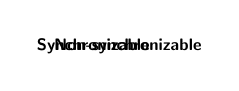
\begin{tikzpicture}[scale=1.5,font=\bf \sffamily \fontsize{6}{6}\selectfont]


\node [] (A)  {\Gtwo};
\node [] (aa) at (A.south)  {Synchronizable};

\node [anchor=west] (B) at ([xshift=.05in]A.east)  {\Gone};

\node [] (bb) at (B.south)  {Non-synchronizable};



\end{tikzpicture}
\vspace{-20pt}

\captionN{{\bf Synchronizable and non-synchronizable machines.} Identifying contexts is a key step in estimating the entropy rate of stochastic signals sources; and for PFSA generators, this translates to a state-synchronization problem. However, not all PFSAs are synchronizable, $e.g.$, while the top machine is synchronizable, the bottom one is not. Note that  a history of just one symbol suffices to determine the current state in the synchronizable machine (top), while no finite history can do the same in the non-synchronizable machine (bottom). However, we show that a $\epsilon$-synchronizable string always exists (Theorem~\ref{thmepssynchro}).
}\label{figsync} 
\vspace{-15pt}

\end{figure}
% #######################################
% #######################################


\begin{thm}[$\epsilon$-Synchronization of Probabilistic Automata]\label{thmepssynchro}
 For any QSP $\mathcal{H}$ over  $\Sigma$, the PFSA  $\mathcal{P}_\mathcal{H}$ satisfies: 
\cgather{
\forall \epsilon' > 0, \exists x \in \Sigma^\star, \exists\bvec  \in \mathcal{E},  \vert \vert \wp_x -\bvec \vert \vert_\infty \leqq \epsilon'\label{eqsync}
}
%where the norm used is unimportant.
\end{thm}
% 
% \begin{proof}
%  See Appendix.
% \end{proof}

\begin{proof}
See \cite{CLx}.
\end{proof}
Theorem~\ref{thmepssynchro} induces the notion of  $\epsilon$-synchronizing strings, and guarantees their existence for arbitrary PFSA.
%\vspace{5pt}
\begin{defn}[$\epsilon$-synchronizing Strings]\label{defepsilonsynchro}
  A  string $x\in \Sigma^\star$ is $\epsilon$-synchronizing for a PFSA if:
\cgather{
\exists\bvec  \in \mathcal{E}, \vert \vert \wp_x -\bvec  \vert \vert_\infty \leqq \epsilon
}
%The norm used is unimportant.
\end{defn}

Theorem~\ref{thmepssynchro} is an existential result, and  does not yield an algorithm for computing synchronizing strings (See Theorem~\ref{thmderivheap}). 
We may  estimate an asymptotic upper bound on such a search.

\begin{cor}[To Theorem~\ref{thmepssynchro}]\label{corsynchrodepth}
At most $O(1/\epsilon)$ strings from the lexicographically ordered set of all strings over the given alphabet need to be analyzed to find an $\epsilon$-synchronizing string.
\end{cor}
% \begin{proof}
%  See Appendix.
% \end{proof}
\begin{proof}
See \cite{CLx}.
\end{proof}
%
%We next introduce the notion of symbolic derivatives:
\subsubsection*{Symbolic Derivatives}
Computation of $\epsilon$-synchronizing strings requires the notion of symbolic derivatives. Note that, PFSA states  are not  observable; we observe  symbols generated from hidden states. A symbolic derivative at a given string  specifies the distribution of the next symbol over the alphabet.

\begin{notn}
We denote the set of probability distributions 
over a finite  set of cardinality $k$ as $\mathscr{D}(k)$. 
\end{notn}

%First, we specify a count function.
\begin{defn}[Symbolic Count Function]\label{defcount}
 For a string $s$ over  $\Sigma$, the count function $\#^s: \Sigma^\star \rightarrow \mathbb{N}\cup \{0\}$,  counts the number of times a particular substring occurs in $s$. The count is overlapping, $i.e.$, in a string $s=0001$, we count the number of occurrences of $00$s as $\underline{00}01$ and $0\underline{00}1$, implying $\#^s 00 =2$.
\end{defn}

\begin{defn}[Symbolic Derivative]\label{defsymderivative}
 For a string $s$  generated by a QSP over $\Sigma$, the symbolic derivative  $\phi^s:\Sigma^\star \rightarrow \mathscr{D}(\vert \Sigma\vert -1)$ is defined:
\vspace{-5pt}
\cgather{
\phi^s(x) \big \vert_i = \frac{\#^s x\sigma_i}{\sum_{\sigma_i \in \Sigma }\#^s x\sigma_i}
}
Thus,  $\forall x \in \Sigma^\star, \phi^s(x)$ is a probability distribution over $\Sigma$. $\phi^s(x)$ is referred to as the symbolic derivative at $x$.
\end{defn}

Note that  $\forall q_i \in Q$, $\pitilde$  induces a  probability distribution over $\Sigma$ as  $[\pitilde(q_i,\sigma_1), \cdots , \pitilde(q_i,\sigma_{\vert \Sigma \vert})]$. We denote this as $\pitilde(q_i,\cdot)$.

We next show that the symbolic derivative at $x$ can be used to estimate this distribution for $q_i = [x]$, provided $x$ is $\epsilon$-synchronizing.
%\vspace{5pt}
\begin{thm}[$\epsilon$-Convergence]\label{thmsymderiv} If $x \in \Sigma^\star$ is $\epsilon$-synchronizing, then:
 \cgather{
\forall \epsilon > 0,  \lim_{\vert s \vert \rightarrow \infty}\vert \vert \phi^s(x) -\pitilde([x],\cdot)\vert \vert_\infty \leqq_{a.s} \epsilon\label{eqsync2} 
% 
}
\end{thm}
\begin{proof}
See \cite{CLx}.
\end{proof}
\subsubsection*{Computation of  $\epsilon$-synchronizing Strings}
Next we describe identification of  $\epsilon$-synchronizing strings given a sufficiently long observed string ($i.e.$ a sample path) $s$. Theorem~\ref{thmepssynchro}  guarantees existence, and Corollary~\ref{corsynchrodepth} establishes that $O(1/\epsilon)$ substrings need to be analyzed till we encounter an $\epsilon$-synchronizing string.
% 
%  What these results do not tell us, is how we would determine that we have indeed found such a string; since we do not have the PFSA (which is what we are trying to construct), there is no  direct way of checking for $\epsilon$-synchronization. 
These  do not provide an executable algorithm, which arises from  
an inspection of the geometric structure of the set of probability vectors over $\Sigma$, obtained by constructing $\phi^s(x)$ for different choices of the candidate string $x$.
% , offers a solution.

% Recall that the set $\mathscr{D}(\vert \Sigma \vert -1)$ denotes the set of probability distributions over $\Sigma$.
% Also, for a set 

\begin{defn}[Derivative Heap]\label{defderivheap}
  Given a string $s$ generated by a QSP, a derivative heap $\mathcal{D}^s: 2^{\Sigma^\star} \rightarrow \mathscr{D}(\vert \Sigma \vert -1)$ is the set of probability distributions over $\Sigma$ calculated for a  subset of strings  $L \subset \Sigma^\star$ as:
\cgather{
\mathcal{D}^s(L) = \big \{ \phi^s(x): x \in L \subset \Sigma^\star\big \}
}
%  
\end{defn}
% #######################################
\begin{lem}[Limiting Geometry]\label{lemlimderiv}
 Let us define:
\cgather{
\mathcal{D}_\infty = \lim_{\vert s \vert \rightarrow \infty }\lim_{L \rightarrow \Sigma^\star} \mathcal{D}^s(L)
}
If $\mathscr{U}_\infty$ is the convex hull of $\mathcal{D}_\infty$, and $u$ is a vertex of $\mathscr{U}_\infty$, then 
\cgather{
\exists q \in Q, \textrm{such that } u=\pitilde(q,\cdot)
}
\end{lem}

\begin{proof}
 Recalling Theorem~\ref{thmsymderiv}, the result follows from noting that any element of $\mathcal{D}_\infty$ is a convex combination of elements from the set $\{\pitilde(q_1,\cdot), \cdots , \pitilde(q_{\vert Q\vert},\cdot)  \}$.
\end{proof}

Lemma~\ref{lemlimderiv} does not claim that the number of vertices of the convex hull of $\mathds{D}_\infty$ equals the number of states, but that every vertex  corresponds to a state.  We cannot generate $\mathcal{D}_\infty$  since we 
have a finite observed string $s$, and we can  calculate $\phi^s(x)$ for a finite number of  $x$. Instead, we show that  choosing a string corresponding to the vertex of the convex hull of the  heap, constructed by considering $O(1/\epsilon)$ strings, gives us an $\epsilon$-synchronizing string with high probability.

\begin{thm}[Derivative Heap Approx.]\label{thmderivheap}
 For  $s$ generated by a QSP, let $\mathcal{D}^s(L)$ be computed with $L=\Sigma^{O(log(1/\epsilon))}$. If for  $x_0 \in \Sigma^{O(log(1/\epsilon))}$,  $\phi^s(x_0)$  is a vertex of the convex hull of $\mathcal{D}^s(L)$, then 
\cgather{
Prob(\textrm{$x_0$ is not $\epsilon$-synchronizing}) \leqq e^{-\vert s \vert \epsilon p_0}
}
 where $p_0$ is the probability of encountering  $x_0$ in $s$.
\end{thm}

% \begin{proof}
%  The result follows from Sanov's Theorem~\cite{Cs84} for convex set of probability distributions. See Appendix for details.
% \end{proof}
% 
\begin{proof}
See \cite{CLx}.
\end{proof}
%%%%%
\subsection*{Entropy Rate for PFSA-generated Processes}
Given the  PFSA model, the entropy rate is easily computable.
\begin{thm}[Entropy Rate For PFSA]\label{thmentropyratepfsa}
The entropy rate $H(G)$, in bits,  for the  QSP generated by  a PFSA $G=(Q,\Sigma,\delta,\pitilde)$ is given by:
\cgather{\label{eqnEPFSA}
H(G) = \sum_{i=1}^{\vert Q\vert} \wp_\lambda\big \vert_i \sum_{\sigma_j \in \Sigma} \pitilde(q_i,\sigma_j) \log\pitilde(q_i,\sigma_j)
}
where the base of the logarithms is $2$.
\end{thm}
\begin{proof}
See \cite{CLx}.
\end{proof}
If the underlying PFSA model is not available, and we have only  a symbolic stream generated by a QSP, then  Eq.~\eqref{eqnEPFSA} cannot be directly employed to estimate the entropy rate. In that case, one possibility is to  first infer the hidden PFSA  using the algorithm reported in \cite{CL12g}, and then estimate the entropy rate from Eq.~\eqref{eqnEPFSA}. However, if we are only interested in the latter, then we do not need to infer the complete generative model; and there exists a more parsimonious approach to estimate the entropy rate directly. 
%
%#########################################################
%#########################################################
%#########################################################
\def\TOL{\textrm{\scshape Count}_\textrm{total}}
\def\Tol{\textrm{\scshape Count}_\textrm{map}}
\def\Num{\textrm{\scshape Num}}
\begin{algorithm}[t]\sffamily \fontsize{7}{8}\selectfont
%\SetCommentSty{textbf}
\SetKw{BRK}{break}
\DontPrintSemicolon
\KwIn{Data sequence $s$ over alphabet $\Sigma$, $\epsilon$,  Confidence level $\alpha$ }
\KwOut{ Entropy rate $\mathbf{h}$, Uncertainty $\mathbf{E}$ at specified confidence level }
%Compute $\epsilon$-synchronizing string $x_0$\;
\BlankLine

Initialize $h=0$\;
Initialize $\TOL = 0$\;
Initialize $\Tol = \varnothing$  \color{Red4}
 \tcc*[f]{\texttt{ \fontsize{6}{6}\selectfont hashtable with keys as  probability distributions, $\phantom{xxxxxxxxxx.xxxxxxxxxxxxxxx}$  and values as doubles}}\color{black}\;
Set $ C_0 = (8/e+8/e^2)(\vert \Sigma \vert -1)$,   $C_1  = 2 / \log^2 \vert \Sigma \vert $\;
Set $N_{\mathrm{min}} = 10$\color{Red4}\tcc*[f]{ \texttt{ \fontsize{6}{6}\selectfont Any small integer suffices (See Section~\ref{secimpl})}}\color{black}\;
\BlankLine
\rule{.945\columnwidth}{1pt}
%\BlankLine
\color{DodgerBlue4}
\tcc*[f]{\scriptsize I. $\epsilon$-synchronization String Identification}\;\color{black}
\BlankLine


\ForEach{$x \in \Sigma^{\log(1/\epsilon)}_+$}{
$D[x] \longleftarrow \phi^s(x) $\;
}

 $A \longleftarrow \{x': \textrm{$D[x']$ is on the convex hull of the set of values in hashtable $D$} \}$\;
 $x_0 \longleftarrow \argmax_{x \in A} \#^sx$\color{Red4}\tcc*[f]{ \texttt{ \fontsize{6}{6}\selectfont $\epsilon$-synchronization string}}\color{black} \;
$p_0  \longleftarrow (\#^sx_0 )\vert s \vert $ \color{Red4}\tcc*[f]{ \texttt{ \fontsize{6}{6}\selectfont Occurrence prob. of $\epsilon$-synchronization string}}\color{black}\;
%\BlankLine
\rule{.945\columnwidth}{1pt}
%\BlankLine
\color{DodgerBlue4}
\tcc*[f]{\scriptsize II. Entropy Rate Estimatation}\;\color{black}
\BlankLine

Select  $\ND \subset \Sigma^\star $ with length $\ell$  strings drawn with probability $\frac{1}{\vert \Sigma \vert^\ell}$\;
\color{Red4}\tcc*[h]{ \texttt{ \fontsize{6}{6}\selectfont $\vert \ND \vert \sim 10^7 \log^2 \vert \Sigma \vert$ sufficient for negligible  uncertainty contribution}}\color{black}\;
%\BlankLine
\ForEach{$x \in \ND$}{
\eIf{$\#^s x_0x > N_{\mathrm{min}}$}{
Compute $u \longleftarrow \phi^s(x_0x)$\color{Red4}\tcc*[f]{ \texttt{ \fontsize{6}{6}\selectfont Symbolic derivative at $x_0x$}}\color{black}\;
%
\eIf{$\exists \textbf{ key } v \in \Tol \textrm{ s.t. }  \| u - v \|_\infty \leqq \epsilon $}{
$\Tol[v] \longleftarrow \Tol [v] +1$\;
}{
Set $\Tol[u] = 1$\;
}
%
$\TOL \longleftarrow \TOL +1$\;
}{
Delete $x$ from $\ND$\;
}
}

\ForEach{$\mathrm{key} \ v \in \Tol$}{
$\mathbf{h} \longleftarrow \mathbf{h} + \left (\dfrac{\Tol[v]}{\TOL}  \times H(v)\right )$\color{Red4}\tcc*[f]{ \texttt{ \fontsize{6}{6}\selectfont $H(v)$: entropy of $v$}}\color{black}\;
}
%\BlankLine
\rule{.945\columnwidth}{1pt}
%\BlankLine
\color{DodgerBlue4}
\tcc*[f]{\scriptsize III. Uncertainty Estimation}\;\color{black}
\BlankLine

$\epsilon_\star \longleftarrow \min \epsilon_0$ satisfying:
$ \alpha+  C_0 \frac{1+\epsilon^2_0}{\vert s \vert \epsilon^{3}_0} + 2 e^{-C_1\vert \ND \vert  \epsilon^{2}_0 } + e^{-\epsilon_0 p_0 \vert s \vert} \leqq  1 $\;
$\mathbf{E} \longleftarrow \epsilon_\star + 2 \mathds{B}(\epsilon_\star, \vert \Sigma \vert)$\;
\KwRet $\mathbf{h}$, $\mathbf{E}$\; 
% 
\captionN{Detailed pseudocode for entropy rate estimation}\label{algo1}
\end{algorithm}
%#########################################################
%#########################################################
%#########################################################

%#########################################################
%#########################################################
%% 

First, we need a lemma which bounds the deviation in entropy for deviations in the probability distribution in the discrete case.
\begin{lem}[Bound on Entropy Deviation]\label{lementropydev}
For probability distributions $p,q$ on a finite set $\Sigma$, we have for all $\epsilon \in (0,1)$,
\cgather{
\vert \vert p -q \vert \vert_\infty \leqq \epsilon \Rightarrow \notag \\\vert H(p) - H(q) \vert <  \epsilon' \log \frac{\vert \Sigma \vert-1}{\epsilon'} + (1-\epsilon') \log \frac{1}{1-\epsilon'} \notag\\
\textrm{where } \epsilon' = \left \{ \begin{array}{cl}
\epsilon & \textrm{if } \epsilon \leqq 1 / 2 \\
1 - \epsilon & \textrm{otherwise} 
\end{array}\right. \notag
}
where $H(p),H(q)$ are  entropies for distributions  $p,q$ respectively.
\end{lem}

\begin{proof}
See \cite{CLx}.
\end{proof}
This  bound on entropy deviation for $\infty$-norm bounded deviations in   distribution will be important in the sequel. We denote this as the generalized binary entropy function $\mathds{B}(\epsilon, \vert \Sigma \vert )$.
\begin{defn}[Generalized Binary Entropy Function]\label{defbef}
\cgather{
\mathds{B}(\epsilon, \vert \Sigma \vert ) = \epsilon' \log \frac{\vert \Sigma \vert-1}{\epsilon'} + (1-\epsilon') \log \frac{1}{1-\epsilon'}\\
\textrm{where } \epsilon' = \left \{ \begin{array}{cl}
\epsilon & \textrm{if } \epsilon \leqq 1 / 2 \\
1 - \epsilon & \textrm{otherwise} 
\end{array}\right. \notag
}
\end{defn}

%As a corollary to Lemma~\ref{lementropydev}, we have the following result:
\begin{cor}[To Lemma~\ref{lementropydev}]
Given a symbol stream generated by a PFSA  $G=(Q,\Sigma,\delta,\pitilde)$, and an $\epsilon$-synchronizing string $x_0$, we have:
\cgathers{
\left \vert \lim_{n\rightarrow \infty} \frac{1}{\vert \Sigma^n_+ \vert} \sum_{x \in \Sigma^n_+} \lim_{\vert s \vert \rightarrow \infty}H(\phi^s(x_0 x)) - H(G) \right \vert < \mathds{B}(\epsilon, \vert \Sigma \vert )
}
\end{cor}
%
\begin{proof}
See \cite{CLx}.
\end{proof}
%
Next we modify the Dvoretzky-Kiefer-Wolfowitz inequality, to be applicable to the case where the number of samples drawn is itself a random variable.
%
\begin{lem}[DKW-bound for symbolic derivatives] \label{lemB1} For a string $s$ generated by a PFSA, and a given $\epsilon$-synchronizing string $x_0$:
\cgathers{\forall x \in \Sigma^\star \textrm{ such that  $x_0x$ occurs in  $s$ with probability $\zeta > 0$ },\\
Pr\left  (\left \vert \left \vert \phi^s(x_0x)  -  \lim_{\mathclap{\vert s' \vert \rightarrow \infty}}\phi^{s'}(x_0 x)  \right \vert \right \vert_{\smash{\infty}}  > \epsilon\right ) < 8(1+\frac{1}{e}) e^{-\vert s \vert \zeta \frac{\epsilon^2}{1+\epsilon^2}}
}

\end{lem}
\begin{proof}
See \cite{CLx}.
\end{proof}

\begin{cor}[To Lemma~\ref{lemB1}]\label{corlemB1} For $s$ generated by a PFSA, and an $\epsilon$-synchronizing $x_0$, we have for any $x \in \Sigma^\star$:
\cgathers{
 Pr\left  (  \bigg \vert H(\phi^s(x_0x) )  -  H\left (\lim_{\vert s' \vert \rightarrow \infty}\phi^{s'}(x_0 x)\right )  \bigg \vert  >  \mathds{B}(\epsilon, \vert \Sigma \vert )\right ) \notag \\ <  8\left (1+\frac{1}{e}\right ) e^{-\vert s \vert \zeta \frac{\epsilon^2}{1+\epsilon^2}}}
\end{cor}
%
\begin{proof}
See \cite{CLx}.
\end{proof}
%
%#########################################################
%#########################################################
\begin{thm}[Bound on Entropy Calculation with Finite Samples]\label{thmB1} For any string $x$ generated by a PFSA $G=(Q,\Sigma,\delta,\pitilde)$, and a given $\epsilon$-synchronizing string $x_0$, there exist  $ C_0, C_1$  depending only on the size of the alphabet $\vert \Sigma \vert$, such that, for any independently chosen set of strings  $\ND \subseteqq \Sigma^\star$:
\cgathers{
Pr \Bigg ( \bigg \vert   \frac{1}{\vert\ND \vert} \sum_{\mathclap{\phantom{X} x \in \ND}} H(\phi^s(x_0 x))   - \lim_{n\rightarrow \infty} \frac{1}{\vert \Sigma^{n}_+ \vert} \sum_{x \in \Sigma^{n}_+} \lim_{\mathclap{\phantom{X} \vert s \vert \rightarrow \infty}}H(\phi^s(x_0 x)) \bigg \vert \notag \\ > \mathds{B}(\epsilon, \vert \Sigma \vert ) + \epsilon\Bigg ) \leqq  C_0 \frac{1+\epsilon^2}{\vert s \vert \epsilon^3} + 2 e^{C_1\vert \ND \vert  \epsilon^{2} } 
}
\end{thm}
\begin{proof}
See \cite{CLx}.
\end{proof} 
%%#########################################################
%#########################################################
\begin{figure}[t]
\tikzexternalenable 
\centering
\def\HGT{1.5in}
\def\WDT{2.85in}
\def\SCALE{1}
\def\datafile{Figures/alph27.dat}
\begin{tikzpicture}[font=\bf \sffamily \fontsize{6}{6}\selectfont]
 \pgfplotsset{every axis legend/.append style={
at={(0.265,0.625)},
anchor=south}}
\begin{semilogxaxis}[ title={(a) Alphabet Size = $27$}, title style={yshift=-.1in},legend cell align=left,
legend style={ xshift=1in, yshift=-.1in, draw=white, fill= gray, fill opacity=0.2, 
text opacity=1,},
axis line style={black, opacity=0.5,  thick, rounded corners=0pt},
axis on top=false, 
scale=1,grid style={dashed, gray!40},
enlargelimits=false, 
width=\WDT, 
height=\HGT,     % size of the image
% xmin=100
,ymax=1.5, 
 ymin=0.00001,
% ymax=17,
semithick,grid,
axis background/.style={top color=gray!0,},
xlabel={input length [\# of symbols]},
yticklabel style={xshift=.025in},
ylabel={error [bits / letter]},
ylabel style={yshift=-.2in},
 xlabel style={yshift=.1in},
    scaled x ticks = false,
      x tick label style={/pgf/number format/fixed,
      /pgf/number format/1000 sep = \thinspace % Optional if you want to replace comma as the 1000 separator 
      }
  ];
% 
%\input{Figures/beta.tex}
%\node at (axis cs:2.75,.25) {0.25}; 
%\node at (axis cs:3.75,.074) {0.074};
%\node at (axis cs:4.75,.023) {0.023};

%\addplot[ thick, mark options={opacity=0.8},mark=*,mark size=1.25pt,red,mark options={
%scale=1.5,fill=green,draw=black
%}]table[x index={0}, y expr=(\thisrowno{1}*\SCALE)]
 % {\datafile};

\addplot[  thick, Red4]table[x index={0}, y expr=(\thisrowno{1}*\SCALE)]
  {\datafile};
\addlegendentry{95\% confidence};

\addplot[  thick, DodgerBlue4]table[x index={2}, y expr=(\thisrowno{3}*\SCALE)]
  {\datafile};
\addlegendentry{99\% confidence};


\node [circle, fill=none, draw=black, inner sep=1pt] (a) at (axis cs:5e6, .9) {};
\draw[gray, thin](a -| current plot begin) -- (a) node [midway,sloped, yshift=0.02in, below, text=black!80, xshift=0.08in, font=\bf \sffamily \fontsize{6}{6}\selectfont] {$0.9$};
\draw[gray, thin]  (a) -- (current plot end -| a) node [midway,sloped, yshift=-0.03in, above, text=black!80, xshift=0.03in, font=\bf \sffamily \fontsize{6}{6}\selectfont] {$5\times 10^6$};

\end{semilogxaxis}
\end{tikzpicture}




\vspace{2pt}
 

\def\SCALE{1}
\def\datafile{Figures/alph2.dat}
\begin{tikzpicture}[font=\bf \sffamily \fontsize{6}{6}\selectfont]
 \pgfplotsset{every axis legend/.append style={
at={(0.265,0.625)},
anchor=south}}
\begin{semilogxaxis}[ title={(b) Alphabet Size = $2$}, title style={yshift=-.1in},legend cell align=left,
legend style={ xshift=1in, yshift=-0.1in, draw=white, fill= gray, fill opacity=0.2, 
text opacity=1,},
axis line style={black, opacity=0.5,  thick, rounded corners=0pt},
axis on top=false, 
scale=1,grid style={dashed, gray!40},
enlargelimits=false, 
width=\WDT, 
height=\HGT,     % size of the image
% xmin=100
,ymax=.95, 
 ymin=0.00001,
% ymax=17,
semithick,grid,
axis background/.style={top color=gray!0,},
xlabel={input length [\# of symbols]},
yticklabel style={xshift=.025in},
ylabel={error [bits / letter]},
ylabel style={yshift=-.2in},
 xlabel style={yshift=.1in},
    scaled x ticks = false,
      x tick label style={/pgf/number format/fixed,
      /pgf/number format/1000 sep = \thinspace % Optional if you want to replace comma as the 1000 separator 
      } 
  ];
% 
%\input{Figures/beta.tex}
%\node at (axis cs:2.75,.25) {0.25};
%\node at (axis cs:3.75,.074) {0.074};
%\node at (axis cs:4.75,.023) {0.023};

%\addplot[ thick, mark options={opacity=0.8},mark=*,mark size=1.25pt,red,mark options={
%scale=1.5,fill=green,draw=black
%}]table[x index={0}, y expr=(\thisrowno{1}*\SCALE)]
 % {\datafile};

\addplot[  thick, Red4]table[x index={0}, y expr=(\thisrowno{1}*\SCALE)]
  {\datafile};
\addlegendentry{95\% confidence};

\addplot[  thick, DodgerBlue4]table[x index={2}, y expr=(\thisrowno{3}*\SCALE)]
  {\datafile};
\addlegendentry{99\% confidence};


\node [circle, fill=none, draw=black, inner sep=1pt] (a) at (axis cs:5e6, .22) {};
\draw[gray, thin](a -| current plot begin) -- (a) node [midway,sloped, yshift=-0.02in, above, text=black!80, xshift=0.08in, font=\bf \sffamily \fontsize{6}{6}\selectfont] {$0.22$};
\draw[gray, thin]  (a) -- (current plot end -| a) ;


\end{semilogxaxis}
\end{tikzpicture}


\vspace{-10pt}

\captionN{\textbf{Uncertainty bounds  for different alphabet sizes.} Note for a data length of $5\times 10^6$, we have an uncertainty of $0.9$ bits at $95 \%$ confidence for a $27$ letter alphabet (plate (a)); the corresponding uncertainty for a binary alphabet is $0.22$ bits (plate(b)). }\label{figBND}
\vspace{-18pt}

\end{figure}
%#########################################################
%#########################################################
\begin{thm}[Main Theorem]\label{thmB2}
Given a finite string $s$ generated by a PFSA  $G=(Q,\Sigma,\delta,\pitilde)$, and a string  $x_0 \in \Sigma^\star$ satisfying the pre-conditions described in Theorem~\ref{thmderivheap}, 
%and an $\epsilon$-synchronizing string $x_0$, 
we have for  any independently chosen set of strings $\ND \subseteqq \Sigma^\star$:
\cgather{
Pr \Bigg ( \bigg \vert   \frac{1}{\vert \ND \vert} \sum_{\mathclap{x \in \ND}} H(\phi^s(x_0 x))   - H(G) \bigg \vert > \epsilon +2\mathds{B}(\epsilon, \vert \Sigma \vert ) \Bigg ) \notag \\ \leqq C_0 \frac{1+\epsilon^2}{\vert s \vert \epsilon^{3}} + 2 e^{-C_1\vert \ND \vert  \epsilon^{2} } + e^{-\epsilon p_0 \vert s \vert} \label{eqBND}
}
where $
C_0=(8/e+8/e^2)(\vert \Sigma \vert -1)$,    $C_1=2 / \log^2 \vert \Sigma \vert$ and $p_0$ is the non-zero occurrence probability of $x_0$ in $s$.
\end{thm}
\begin{proof}
See \cite{CLx}.
\end{proof}
%#########################################################
%#########################################################
\begin{figure*}[t] 
\tikzexternalenable 
\centering
% ##########################################################
\newcommand{\Vdist}{.5in}
\def\COL{black!50}
\def\COLA{Red4!20!black}
\def\COLB{Red4!20!black}
\def\COLC{Red4!20!black}
\def\GCOL{gray!0}

\definecolor{blcol}{RGB}{150,150,250}
\definecolor{murcol}{RGB}{255,150,150}
\definecolor{healcol}{RGB}{150,235,150}
\definecolor{colzeta}{RGB}{250,250,200}
\definecolor{leftpcol}{RGB}{200,255,200}
\definecolor{rightpcol}{RGB}{200,200,255}
\definecolor{boxcol}{RGB}{210,200,200}
\definecolor{linecol}{RGB}{200,180,180}
\definecolor{colplus}{RGB}{235,220,220}
\definecolor{colinv}{RGB}{200,220,255}
\definecolor{cof}{RGB}{219,144,71}
\definecolor{pur}{RGB}{200,200,200}
\definecolor{greeo}{RGB}{91,173,69}
\definecolor{greet}{RGB}{52,111,72}
 \definecolor{nodecol}{RGB}{180,180,220}
 \definecolor{nodeedge}{RGB}{140,148,155}
  \definecolor{nodecolb}{RGB}{220,180,180}
  \definecolor{nodecolc}{RGB}{180,220,180}
  \definecolor{nodecolcD}{RGB}{100,160,100}
  \definecolor{nodecolW}{RGB}{190,190,190}
  \definecolor{edgecol}{RGB}{60,60,80}
 \definecolor{nodecolD}{RGB}{140,140,180}
  \definecolor{nodecolbD}{RGB}{180,140,140}
 % ##########################################################
% ##########################################################
\tikzset{srule/.style={ semithick, opacity=.8, Red1, text opacity=1, text=gray}}
\tikzset{axstyle/.style={ black, opacity=1,  thick, rounded corners=0pt}}
\tikzset{%
fshadow/.style={      preaction={
         fill=black,opacity=.2,
         path fading=circle with fuzzy edge 20 percent,
         transform canvas={xshift=1mm,yshift=-1mm}
       }}
}
% ##########################################################
% ##########################################################
\tikzset{oplus/.style={path picture={% 
      \draw[black]
       (path picture bounding box.south) -- (path picture bounding box.north) 
       (path picture bounding box.west) -- (path picture bounding box.east);
      }}} 
% ##########################################################
% ##########################################################
\tikzset{%
  highlight/.style={draw=Red4,rectangle,rounded corners=1pt, opacity=1,fill=gray!10,thick,inner sep=-1.25pt,on background layer,fill opacity=.3}
}
\tikzset{%
  highlightg/.style={draw=DodgerBlue4,rectangle,rounded corners=1pt, opacity=1,fill=gray!10,thick,inner sep=-1.25pt,on background layer,fill opacity=.3}
}
% 
% ##################################
\newcommand{\Gone}{%
\begin{tikzpicture}[->,>=stealth',shorten >=1pt,auto,node distance=1.2cm,
                    semithick,scale=.65,font=\bf\fontsize{6}{6}\selectfont]
  \tikzstyle{every state}=[fill=nodecol,draw=nodeedge,text=black,minimum size=3, text width=2,scale=1,fshadow]
  \node[state] (A)         []           {$\mspace{-6mu}q_0$};
  \node[state]         (B) [right of=A] {$\mspace{-6mu}q_1$};
  \path (A) edge   [draw=edgecol,bend left]           node {$\sigma_1\vert 0.15$} (B)
        (A) edge [draw=edgecol,in=120,out=60,loop,left] node [xshift=-.1in,yshift=-.1in]{$\sigma_0\vert 0.85$} (A)
        (B) edge [draw=edgecol,in=60,out=120,loop,right] node [xshift=.1in,yshift=-.1in]{$\sigma_0\vert 0.25$} (B)
            edge   [draw=edgecol,bend left]           node {$\sigma_1\vert 0.75$} (A);
\end{tikzpicture}
}
% ##################################
% ##################################
\newcommand{\Gtwo}{%
\begin{tikzpicture}[->,>=stealth',shorten >=1pt,auto,node distance=1.2cm,
                    semithick,scale=.65,font=\bf\fontsize{6}{6}\selectfont]
  \tikzstyle{every state}=[fill=nodecolb,draw=nodeedge,text=black,minimum size=3, text width=2,scale=1,fshadow]
  \node[state] (A)         []           {$\mspace{-6mu}q_0$};
  \node[state]         (B) [right of=A] {$\mspace{-6mu}q_1$};
  \path (A) edge   [draw=edgecol,bend left]           node {$\sigma_1\vert 0.15$} (B)
        (A) edge [draw=edgecol,in=120,out=60,loop,left] node [xshift=-.1in,yshift=-.1in]{$\sigma_0\vert 0.85$} (A)
        (B) edge [draw=edgecol,in=60,out=120,loop,right] node [xshift=.1in,yshift=-.1in]{$\sigma_1\vert 0.75$} (B)
            edge   [draw=edgecol,bend left]           node {$\sigma_0\vert 0.25$} (A);
\end{tikzpicture}
}
% ##################################




\def\HGT{1.78in}
\def\WDT{2.3in}
\def\SCALE{1}
%#################################
%##################################
\def\datafileA{Figures/kjb.dat}
\def\datafileB{Figures/kjbCL.dat}
\def\datafileC{Figures/shks.dat}
\def\datafileD{Figures/shksCL.dat}
\def\datafileE{Figures/chaos1p7499.dat}
\def\datafileF{Figures/chaos1p2.dat}
\def\datafileG{Figures/pfsaS1.dat}
\def\datafileH{Figures/pfsaM1.dat}
\begin{tikzpicture}[font=\bf \sffamily \fontsize{6}{6}\selectfont]
 \pgfplotsset{every axis legend/.append style={
at={(0.265,0.625)},
anchor=south}}
%#################################
%##################################
%############## TEXT #############
%##################################
%#################################
%##################################
\begin{axis}[ name=A, title={{\normalsize (a)} King James' Bible}, title style={yshift=-.1in},legend cell align=left,
legend style={   legend pos=north east,, draw=white, fill= gray, fill opacity=0.25, 
text opacity=1,},
axis line style={axstyle},
axis on top=false, 
scale=1,grid style={dashed, gray!60},
enlargelimits=true, 
width=\WDT, 
height=\HGT,     % size of the image
thick,grid,
axis background/.style={top color=\GCOL,},
xlabel={input length [\# of symbols $\times 10^6$]},
yticklabel style={xshift=.025in},
ylabel={entropy rate [bits / letter]},
ylabel style={yshift=-.35in},
 xlabel style={yshift=.1in},
  ];
\draw[srule ] (axis cs:\pgfkeysvalueof{/pgfplots/xmin},1) -- (axis cs:\pgfkeysvalueof{/pgfplots/xmax},1) node [midway, xshift=-.35in,above] {Shannon Estimate};

\addplot[   thick, \COL]table[x expr=(\thisrowno{0}* 0.000001), y expr=(\thisrowno{1}*\SCALE)]
  {\datafileA};
\addlegendentry{state-of-art};

\addplot[  thick, \COLA, ]table[x expr=(\thisrowno{0}* 0.000001), y expr=(\thisrowno{1}*\SCALE)]
  {\datafileB};
\addlegendentry{this-paper};
\end{axis}
%#################################
%##################################
\begin{axis}[ name=B, at=(A.south), anchor= north, yshift=-.5in, title={{\normalsize (b)} Shakespeare Collected Works}, title style={yshift=-.1in},legend cell align=left,
legend style={  legend pos=north east, draw=white, fill= gray, fill opacity=0.25, 
text opacity=1,},
axis line style={axstyle},
axis on top=false, 
scale=1,grid style={dashed, gray!60},
enlargelimits=true, 
width=\WDT, 
height=\HGT,     % size of the image
thick,grid,
axis background/.style={top color=\GCOL,},
xlabel={input length [\# of symbols $\times 10^6$ ]},
yticklabel style={xshift=.025in},
ylabel={entropy rate [bits / letter]},
ylabel style={yshift=-.35in},
 xlabel style={yshift=.1in},
  ];
\draw[srule] (axis cs:\pgfkeysvalueof{/pgfplots/xmin},1) -- (axis cs:\pgfkeysvalueof{/pgfplots/xmax},1) node [midway,below] {Shannon Estimate};

\addplot[ thick, \COL]table[x expr=(\thisrowno{0}* 0.000001), y expr=(\thisrowno{1}*\SCALE)]
  {\datafileC};
\addlegendentry{state-of-art};

\addplot[  thick, \COLA]table[x expr=(\thisrowno{0} * 0.000001), y expr=(\thisrowno{1}*\SCALE)]
  {\datafileD};
\addlegendentry{this-paper};
\end{axis}
%#################################
%##################################
%#################################
%##################################
%########### CHAOTIC SYSTEMS ######
%##################################
%#################################
%##################################
\def\WDT{2.3in}
\begin{axis}[ name=C,at=(A.east), anchor= west, xshift=0.5in,title={{\normalsize (c)} Map $\displaystyle x_{n+1} = 1 - rx_{n}^2$, with  $r=1.7499$ }, title style={yshift=-.1in},legend cell align=left,
legend style={   legend pos=north east,, draw=white, fill= gray, fill opacity=0.25, 
text opacity=1,},
axis line style={axstyle},
axis on top=false, 
scale=1,grid style={dashed, gray!60},
enlargelimits=true, 
width=\WDT, 
height=\HGT,     % size of the image
thick,grid,
axis background/.style={top color=\GCOL,},
xlabel={input length [\# of symbols]},
yticklabel style={xshift=.025in},
ylabel={entropy rate [bits / letter]},
ylabel style={yshift=-.22in},
 xlabel style={yshift=.1in},
     scaled x ticks = false,
      x tick label style={/pgf/number format/fixed,
      /pgf/number format/1000 sep = \thinspace % Optional if you want to replace comma as the 1000 separator 
      } ];
\draw[ srule] (axis cs:\pgfkeysvalueof{/pgfplots/xmin},0.2779) -- (axis cs:\pgfkeysvalueof{/pgfplots/xmax},0.2779) node [midway,below] {Theoretical value};

\addplot[   thick, \COL]table[x expr=(\thisrowno{0}* 1), y expr=(\thisrowno{4}*\SCALE)]
  {\datafileE};
\addlegendentry{LZ-compression};

\addplot[  thick, \COLB]table[x expr=(\thisrowno{0}* 1), y expr=(\thisrowno{1}*\SCALE)]
  {\datafileE};
\addlegendentry{this-paper};
\end{axis}
%#################################
%##################################
\begin{axis}[ name=D, at=(C.south), anchor= north, yshift=-.5in, title={{\normalsize (d)} Map $\displaystyle x_{n+1} = 1 - rx_{n}^2$, with  $r=1.75$}, title style={yshift=-.1in},legend cell align=left,
legend style={  legend pos=north east, draw=white, fill= gray, fill opacity=0.25, 
text opacity=1,},
axis line style={axstyle},
axis on top=false, 
scale=1,grid style={dashed, gray!60},
enlargelimits=true, 
width=\WDT, 
height=\HGT,     % size of the image
thick,grid,
ymin=-0.15,
axis background/.style={top color=\GCOL,},
xlabel={input length [\# of symbols ]},
yticklabel style={xshift=.025in},
ylabel={entropy rate [bits / letter $\times 0.01$]},
ylabel style={yshift=-.22in},
 xlabel style={yshift=.1in},
     scaled x ticks = false,
      scaled y ticks = false,
     x tick label style={/pgf/number format/fixed,
      /pgf/number format/1000 sep = \thinspace % Optional if you want to replace comma as the 1000 separator 
      } ];
\draw[ srule] (axis cs:\pgfkeysvalueof{/pgfplots/xmin},0) -- (axis cs:\pgfkeysvalueof{/pgfplots/xmax},0) node [midway,below] {Theoretical value};

\addplot[ thick, \COL]table[x expr=(\thisrowno{0}* 1), y expr=(\thisrowno{4}*100)]
  {\datafileF};
\addlegendentry{LZ-compression};

\addplot[  thick, \COLB]table[x expr=(\thisrowno{0} * 1), y expr=(\thisrowno{1}*100)]
  {\datafileF};
\addlegendentry{this-paper};
\end{axis}
%#################################
%##################################
%#################################
%##################################
%########### PFSA S1 and M1 ######
%##################################
%#################################
%##################################
%#################################
%##################################
\def\WDT{2.4in}
\begin{axis}[ name=E,at=(C.east), anchor= west, xshift=0.5in,title={{\normalsize (e)} Non-synchronizable Stochastic process  }, title style={yshift=-.1in},legend cell align=left,
legend style={   legend pos=north east,, draw=white, fill= gray, fill opacity=0.25, 
text opacity=1,},
axis line style={axstyle},
axis on top=false, 
scale=1,grid style={dashed, gray!60},
enlargelimits=true, 
width=\WDT, 
xmax=30000,
ymin=0.5,
height=\HGT,     % size of the image
thick,grid,
axis background/.style={top color=\GCOL,},
xlabel={input length [\# of symbols]},
yticklabel style={xshift=.025in},
ylabel={entropy rate [bits / letter]},
ylabel style={yshift=-.22in},
 xlabel style={yshift=.1in},
     scaled x ticks = false,
      x tick label style={/pgf/number format/fixed,
      /pgf/number format/1000 sep = \thinspace % Optional if you want to replace comma as the 1000 separator 
      } ];
\draw[ srule] (axis cs:\pgfkeysvalueof{/pgfplots/xmin},0.6434) -- (axis cs:\pgfkeysvalueof{/pgfplots/xmax},0.6434) node [midway,above] {Theoretical value};

\addplot[   thick, \COL]table[x expr=(\thisrowno{0}* 1), y expr=(\thisrowno{4}*\SCALE)]
  {\datafileG};
\addlegendentry{LZ-compression};

\addplot[  thick, \COLC]table[x expr=(\thisrowno{0}* 1), y expr=(\thisrowno{1}*\SCALE)]
  {\datafileG};
\addlegendentry{this-paper};
\end{axis}
%#################################
%##################################
\begin{axis}[ name=F, at=(E.south), anchor= north, yshift=-.5in, title={{\normalsize (f)} Synchronizable Stoachastic Process}, title style={yshift=-.1in},legend cell align=left,
legend style={  legend pos=north east, draw=white, fill= gray, fill opacity=0.25, 
text opacity=1,},
axis line style={axstyle},
axis on top=false, 
scale=1,grid style={dashed, gray!60},
enlargelimits=true, 
width=\WDT, 
height=\HGT,     % size of the image
thick,grid,
ymin=0.6,
ymax=.76,
xmax=30000,
axis background/.style={top color=\GCOL,},
xlabel={input length [\# of symbols ]},
yticklabel style={xshift=.025in},
ylabel={entropy rate [bits / letter]},
ylabel style={yshift=-.22in},
 xlabel style={yshift=.1in},
     scaled x ticks = false,
      scaled y ticks = false,
     x tick label style={/pgf/number format/fixed,
      /pgf/number format/1000 sep = \thinspace % Optional if you want to replace comma as the 1000 separator 
      } ];
\draw[ srule] (axis cs:\pgfkeysvalueof{/pgfplots/xmin},0.68) -- (axis cs:\pgfkeysvalueof{/pgfplots/xmax},0.68) node [midway,above] {Theoretical value};

\addplot[ thick, \COL]table[x expr=(\thisrowno{0}* 1), y expr=(\thisrowno{4}*1)]
  {\datafileH};
\addlegendentry{LZ-compression};

\addplot[  thick, \COLC]table[x expr=(\thisrowno{0} * 1), y expr=(\thisrowno{1}*1.011)]
  {\datafileH};
\addlegendentry{this-paper};
\end{axis}


\node [ anchor=south, text=\COLA] at ([yshift=.2in]A.north) {\fontsize{9}{9}\selectfont \scshape English Text};

\node [ anchor=south, text=\COLB] at ([yshift=.2in]C.north) {\fontsize{9}{9}\selectfont \scshape Chaotic Dynamical Systems};


\node [ anchor=south, text=\COLC] at ([yshift=.2in]E.north) {\fontsize{9}{9}\selectfont \scshape Finite Memory Stochastic Processes};


\node [anchor=south east] at ([yshift=-.05in, xshift=0.02in]E.south east) {\Gone};
\node [anchor=south east] at ([yshift=-.05in, xshift=0.02in]F.south east) {\Gtwo};

\end{tikzpicture}



\vspace{-9pt}

\captionN{\textbf{Applications.} Plates (a-b): Entropy rate of English text. Shannon's experiment using human subjects  puts the estimate around $1$ bit per letter. We achieve very close estimates. The state-of-the-art plots are replicated from~\cite{shgs96}. Plates (c-d): Entropy rate of sequences generated by a chaotic dynamical system and a binary generating partition. Plates (e-f): Entropy of symbol streams generated by probabilistic automata. Note that even with two states, and a binary alphabet, a non-synchronizable generating process leads to significantly larger errors with the LZ-based approaches.}\label{figTXT}
\vspace{-15pt}

\end{figure*}
%#########################################################
%#########################################################
\begin{rem}
We note the following:
\begin{itemize}
\item For binary alphabets, we have: $
C_0 \simeq 4.03, C_1 = 2
$.
\item Each term on  the RHS of Eq.~\eqref{eqBND} reflects   a specific contribution:
\cgather{
\underbrace{C_0 \frac{1+\epsilon^2}{\vert s \vert \epsilon^{3}}}_{\mathclap{\text{Data-length Dependence}}} + \overbrace{2 e^{-C_1\vert \ND \vert \epsilon^{2} }}^{\mathclap{\text{Dependence on Summation Depth}}} + \underbrace{e^{-\epsilon p_0 \vert s \vert}}_{\mathclap{\text{Synchronization Error Dependence}}}
}
\end{itemize}
\item Eq.~\eqref{eqBND} bounds the maximum uncertainty at a given confidence level, which depends on the alphabet size. The uncertainty relationships for two alphabet sizes ($2$, $27$) are shown in Figure~\ref{figBND}.
\end{rem}
%
\begin{cor}[To Theorem~\ref{thmB2}]
As a function of the length of the observed data string $s$, the upper and lower confidence bands for the estimated entropy rate, with any fixed confidence level, 
converge at a rate $\displaystyle O\left (\frac{\log \vert s \vert }{ \vert s \vert^{1/3}}\right )$.
\end{cor}
\begin{proof}
See \cite{CLx}.
\end{proof}
\subsection*{Algorithmic Implementation}\label{secimpl}
The algorithmic steps for the proposed entropy rate estimation technique is enumerated in Algorithm~\ref{algo1}. The inputs to the algorithm is the data stream $s$, $\epsilon$, and the confidence level $\alpha$ at which the error  estimate is desired.
Importantly, the size of the set of sampled string $\ND$ is not required to be an input; 
if computational effort is not a concern, then the uncertainty contribution from the term involving $\vert \ND \vert$ (See Eq.~\eqref{eqBND}) can be reduced to negligible levels by using a sample set with  
$\vert \ND \vert \simeq \frac{K}{2\epsilon^2} \log^2 \vert \Sigma \vert  
$, which would result in  uncertainty contribution of $\sim e^{-K}$. Using $\vert \ND \vert \simeq 10^7 \log^2 \vert \Sigma \vert$ is generally sufficient to make this factor negligible; smaller sets may be used under computational constraints, which would  lead to  increased uncertainty in the entropy estimate.

Particularly rare strings may accumulate errors, which is prevented in the implementation by ignoring strings that occur too infrequently (Note $N_\mathrm{min}$ in step 5 and step 15 of Algorithm ~\ref{algo1}).
\subsubsection*{Application to English text, Chaotic systems \& Random walks}
We demonstrate  Algorithm~\ref{algo1} in three different applications. 
Our first application is the estimation of the entropy rate of English text. 
Shannon's experimental approach with human subjects~\cite{shannon1951} suggests that English has an entropy of around one bit per letter. However, the  large alphabet size ($26$ letters + space = $27$), makes it computationally hard to verify this value. We apply our algorithm to relatively small corpora: the King James Bible (KJB) (which has a length $\sim 4 \times 10^6$ letters), and the collected works of Shakespeare (SHK, length $\sim 4.8 \times 10^6$ letters). These  particular examples allow direct  comparison against the results reported in \cite{shgs96}. We obtain entropy rates which are significantly closer to the Shannon estimate (See Figure~\ref{figTXT}):  $1.05  \btl$ for KJB, and $1.25  \btl$  for SHK, while Sch{\"u}rmann $\etal$ obtain the corresponding estimates  to be $1.73 \btl$ and $2.13 \btl$. The authors in \cite{shgs96} were able to improve the SHK estimate to  $1.7 \btl$ using the ``ansatz'' mentioned before;  Algorithm~\ref{algo1} yields an improved estimate without any such assumptions. 

Our second application is entropy estimation of sequences produced by chaotic dynamical systems. We use the same iteration map used in \cite{shgs96}: namely $x_{n+1} = 1 - r x^2_n$, and use a binary generating partition at $x=0$. We analyze the  cases
$r=1.7499$ (Figure~\ref{figTXT}(b)) where it is very strongly intermittent, and $r=1.75$ which is the Pomeau-Manneville intermittency point (Figure~\ref{figTXT}(c)). As before, we converge faster in the non-trivial case, and gets very close to the theoretical entropy given by the positive  Lyapunov exponent due to Pesin's identity~\cite{rissanen83}.

Our third application analyzes sequences generated by finite memory ergodic stationary stochastic processes, modeled directly via probabilistic automata (Figure~\ref{figTXT}(e-f)). Thus, we are looking at generalized random walks, Inspite of being  somewhat more contrived compared to the first two applications, we can gain important insights from this example. Even with two states, and with a binary alphabet, LZ-based approaches may perform significantly worse, particularly for short streams with long range dependencies. We note that the PFSA generator used in Figure~\ref{figTXT}(e) is non-synchronizable, $i.e.$, no finite length of observed history tells us definitively what the current state is. Nevertheless, as we showed in Theorem~\ref{thmepssynchro}, the machine is $\epsilon$-synchronizable; and Algorithm~\ref{algo1} performs quite well, converging to the theoretical value with just under $10^4$ symbols. In contrast, the LZ-compression based algorithm has an error of about $17\%$ even after $3 \times 10^4$ symbols. This is discrepancy in performance disappears if the generating process is synchronizable, $e.g.$, if a finite history tells us precisely what the current state is. Indeed with a synchronizable PFSA in Figure~\ref{figTXT}(f) (here, the last symbol is sufficient to fix the current state), the algorithms have comparable performances.

\subsection*{Summary \& Conclusion}\label{sec6}
We delineate a new algorithm for estimating entropy rates of symbol streams,  generated by  hidden ergodic stationary processes. We establish the correctness of the algorithm by exploiting a connection with the theory of probabilistic automata, and that of finite measures on infinite strings. Importantly, we establish a distribution-free limit theorem. Using established results from non-parametric statistics, we show that  entropy  estimate converges at the rate $O(\log \vert s \vert / \sqrt[3]{ \vert s \vert} )$ as a function of the input data length $\vert s \vert$. In consequence, we are able to derive confidence bounds on the  estimate, and dictate the  worst-case data length required to guarantee a specified error bound at a given confidence level. Finally, we demonstrate  that, in terms of data requirements,  the proposed algorithm has superior performance to competing approaches, at least in the case of the chosen applications. 

%\ack{
%This work was supported in part by the ARO Biomathematics program. The content of this paper is solely the responsibility of the authors and does not necessarily represent the official views of the sponsoring organizations.
%}
%##################################################
% #######################################
%#################################################
}%%endALLOWDISPLAYBREAKS  DO NOT REMOVE
%#################################################
 %\fontsize{6}{8}\selectfont
 \bibliographystyle{IEEEtran}
\bibliography{BibLib1} 
\end{document}
